
\documentclass[11pt,twoside]{article}
\usepackage{etex}

\raggedbottom

%geometry (sets margin) and other useful packages
\usepackage{geometry}
\geometry{top=1in, left=1in,right=1in,bottom=1in}
 \usepackage{graphicx,booktabs,calc}
 
\usepackage{listings}


% Marginpar width
%Marginpar width
\newcommand{\pts}[1]{\marginpar{ \small\hspace{0pt} \textit{[#1]} } } 
\setlength{\marginparwidth}{.5in}
%\reversemarginpar
%\setlength{\marginparsep}{.02in}

 
%\usepackage{cmbright}lstinputlisting
%\usepackage[T1]{pbsi}


\usepackage{chngcntr,mathtools}
%\counterwithin{figure}{section}
%\numberwithin{equation}{section}

%\usepackage{listings}

%AMS-TeX packages
\usepackage{amssymb,amsmath,amsthm} 
\usepackage{bm}
\usepackage[mathscr]{eucal}
\usepackage{colortbl}
\usepackage{color}


\usepackage{subfig,hyperref,enumerate,polynom,polynomial}
\usepackage{multirow,minitoc,fancybox,array,multicol}

\definecolor{slblue}{rgb}{0,.3,.62}
\hypersetup{
    colorlinks,%
    citecolor=blue,%
    filecolor=blue,%
    linkcolor=blue,
    urlcolor=slblue
}

%%%TIKZ
\usepackage{tikz}

\usepackage{pgfplots}
\pgfplotsset{compat=newest}

\usetikzlibrary{arrows,shapes,positioning}
\usetikzlibrary{decorations.markings}
\usetikzlibrary{shadows}
\usetikzlibrary{patterns}
%\usetikzlibrary{circuits.ee.IEC}
\usetikzlibrary{decorations.text}
% For Sagnac Picture
\usetikzlibrary{%
    decorations.pathreplacing,%
    decorations.pathmorphing%
}

\tikzstyle arrowstyle=[black,scale=2]
\tikzstyle directed=[postaction={decorate,decoration={markings,
    mark=at position .65 with {\arrow[arrowstyle]{stealth}}}}]
\tikzstyle reverse directed=[postaction={decorate,decoration={markings,
    mark=at position .65 with {\arrowreversed[arrowstyle]{stealth};}}}]
\tikzstyle dir=[postaction={decorate,decoration={markings,
    mark=at position .98 with {\arrow[arrowstyle]{latex}}}}]
\tikzstyle rev dir=[postaction={decorate,decoration={markings,
    mark=at position .98 with {\arrowreversed[arrowstyle]{latex};}}}]

\usepackage{ctable}

%
%Redefining sections as problems
%
\makeatletter
\newenvironment{exercise}{\@startsection 
	{section}
	{1}
	{-.2em}
	{-3.5ex plus -1ex minus -.2ex}
    	{1.3ex plus .2ex}
    	{\pagebreak[3]%forces pagebreak when space is small; use \eject for better results
	\large\bf\noindent{Part 1.\hspace{-1.5ex} }
	}
	}
	%{\vspace{1ex}\begin{center} \rule{0.3\linewidth}{.3pt}\end{center}}
	%\begin{center}\large\bf \ldots\ldots\ldots\end{center}}
\makeatother

%
%Fancy-header package to modify header/page numbering 
%
\usepackage{fancyhdr}
\pagestyle{fancy}
%\addtolength{\headwidth}{\marginparsep} %these change header-rule width
%\addtolength{\headwidth}{\marginparwidth}
%\fancyheadoffset{30pt}
%\fancyfootoffset{30pt}
\fancyhead[LO,RE]{\small Oke}
\fancyhead[RO,LE]{\small Page \thepage} 
\fancyfoot[RO,LE]{\small PS 2} 
\fancyfoot[LO,RE]{\small \scshape CEE 616} 
\cfoot{} 
\renewcommand{\headrulewidth}{0.1pt} 
\renewcommand{\footrulewidth}{0.1pt}
%\setlength\voffset{-0.25in}
%\setlength\textheight{648pt}


\usepackage{paralist}

\newcommand{\osn}{\oldstylenums}
\newcommand{\lt}{\left}
\newcommand{\rt}{\right}
\newcommand{\pt}{\phantom}
\newcommand{\tf}{\therefore}
\newcommand{\?}{\stackrel{?}{=}}
\newcommand{\fr}{\frac}
\newcommand{\dfr}{\dfrac}
\newcommand{\ul}{\underline}
\newcommand{\tn}{\tabularnewline}
\newcommand{\nl}{\newline}
\newcommand\relph[1]{\mathrel{\phantom{#1}}}
\newcommand{\cm}{\checkmark}
\newcommand{\ol}{\overline}
\newcommand{\rd}{\color{red}}
\newcommand{\bl}{\color{blue}}
\newcommand{\pl}{\color{purple}}
\newcommand{\og}{\color{orange!90!black}}
\newcommand{\gr}{\color{green!40!black}}
\newcommand{\nin}{\noindent}
\newcommand{\la}{\lambda}
\renewcommand{\th}{\theta}
\newcommand*\circled[1]{\tikz[baseline=(char.base)]{
            \node[shape=circle,draw,thick,inner sep=1pt] (char) {\small #1};}}

\newcommand{\bc}{\begin{compactenum}[\quad--]}
\newcommand{\ec}{\end{compactenum}}

\newcommand{\n}{\\[2mm]}
%% GREEK LETTERS
\newcommand{\al}{\alpha}
\newcommand{\gam}{\gamma}
\newcommand{\eps}{\epsilon}
\newcommand{\sig}{\sigma}

\newcommand{\p}{\partial}
\newcommand{\pd}[2]{\frac{\partial{#1}}{\partial{#2}}}
\newcommand{\dpd}[2]{\dfrac{\partial{#1}}{\partial{#2}}}
\newcommand{\pdd}[2]{\frac{\partial^2{#1}}{\partial{#2}^2}}
\newcommand{\mr}{\mathbb{R}}
\newcommand{\xs}{x^{*}}
\newenvironment{solution}
{\medskip\par\quad\quad\begin{minipage}[c]{.8\textwidth}}{\medskip\end{minipage}}

\newcommand{\nmfr}[3]{\Phi\left(\frac{{#1} - {#2}}{#3}\right)}
 
%%%%%%%%%%%%%%%%%%%%%%%%%%%%%%%%%%%%%%%%%%%%%%%%%%%
%%%%%%%%%%%%%%%%%%%%%%%%%%%%%%%%%%%%%%%%%%%%%%%%%%%

\begin{document}

\lstset{language=C++,
                basicstyle=\tiny\ttfamily,
                keywordstyle=\color{blue}\ttfamily,
                stringstyle=\color{red}\ttfamily,
                commentstyle=\color{gray}\ttfamily,
                morecomment=[l][\color{gray}]{\#}
}


\thispagestyle{empty}


\nin{\LARGE Problem Set 2 }\hfill{\bf Oke}

\medskip\hrule\medskip

\nin {\small CEE 616: Data Mining and Machine Learning for Engineers
\hfill\textit{ 10.02.2025}}

\nin{\it \small Due October 14, 2025 at 11:59PM. Submit via Canvas.}\\

\nin The standard problems are worth a total of \textbf{93 points}, with \textbf{7 extra credit points} available.

% \subsubsection*{Useful links}
% \begin{itemize}
% \item Defining functions in R: \url{https://www.datamentor.io/r-programming/function/}
% \item Defining functions in Python: \url{https://www.tutorialspoint.com/python/python_functions.htm}
% \item Defining functions in MATLAB: \url{https://www.mathworks.com/help/matlab/ref/function.html}
% \item Logistic regression in MATLAB: \url{https://www.mathworks.com/help/stats/fitglm.html}
% \item LDA in R: \url{https://rpubs.com/ifn1411/LDA}
% \item LDA example in MATLAB: \url{https://www.mathworks.com/help/stats/discriminant-analysis.html}
% \item LDA function and examples in Python: \url{https://scikit-learn.org/stable/modules/generated/sklearn.discriminant_analysis.LinearDiscriminantAnalysis.html}
% \end{itemize}


\subsubsection*{Submission instructions}
There are two options for submission:
\begin{enumerate}
\item JupyterLab Notebook. Please name your notebook as follows: \\ \texttt{<lastname>-<firstname>-PS2.ipynb}
\item R/Python/MATLAB script \textit{and} PDF document with supporting responses.
  Your PDF should have complete responses to all the questions (including all the required plots).
  Your script should be clearly commented, producing all the results and plots you show in your PDF document.
  The filenames should be in a similar format as described above.
\end{enumerate}
Whenever datasets are provided, be sure to leave the relative path and filenames as originally given in order to ensure that your scripts will run properly.
For instance, here, all the data sets are found in the \texttt{data} folder. So, when you call \texttt{read.csv()}, use the relative path, e.g. \texttt{data/Default.csv}.
This way, when you submit your work, you need not include the data. I will have the exact same folder and will be able to run all the scripts as the same path will be referenced.

\eject

% \section*{Problem 1 \quad {\it Classification or regression?}}
% ISLR Exercise 2.2 (p.\ 52). \pts{4pts}

% \section*{Problem 1 \quad {\it Example applications of statistical learning}}
% Draw on your current or future research and/or academic experience to answer the following questions.
% You may want to consult other literature to see some real-world applications of statistical or machine learning.
% Some will be provided in class.

% \begin{enumerate}[\bf (a)]
% \item Describe two real-world applications in which \textit{regression} might be useful. \pts{2pts}
%   Describe the response, as well as the predictors. Is the goal of each application inference or prediction?
%   Explain your answers.

% \item Describe two real-world applications in which \textit{classification} might be useful. \pts{2pts}
%   Describe the response, as well as the predictors. Is the goal of each application inference or prediction?
%   Explain your answers.

% \item Describe two real-world applications in which \textit{cluster analysis} might be useful.   \pts{2pts}
% \end{enumerate}

% \eject

\section*{Problem 1 \quad {\it Logistic regression (20 pts; 2 pts EC)}}

\subsection*{Part 1.1}
In a binary logistic regression with a multiple predictors $\bm x^\intercal = (1, x_1,\ldots,x_D)$, \pts{4}
the logistic function is given by:
\begin{equation}
  \label{eq:1}
  p(\bm x) = \fr{1}{1 + e^{-\bm w^\intercal \bm x}}
\end{equation}
where $\bm w^\intercal = (b, w_1, \ldots, w_D) $.
Using this function, show explicitly that the log-odds or logit function of $p(y=1|\bm x)$ is given by:
\begin{equation}
  \label{eq:2}
  \log\lt(\fr{p(\bm x)}{1 - p(\bm x)}\rt) = \bm w^\intercal \bm x
\end{equation}

% \subsection*{Part 2.2}
% ISLR Exercise 4.6 (a) and (b). \pts{5pts}


\section*{Problem 2 \quad {\it LDA  (13 pts)}}

\begin{enumerate}[\bf (a)]
\item Suppose we have features \pts{8} $x \in \mathbb{R}^D$, a two-class response with class sizes $n_1, n_2$ and the target coded as $\{-n/n_1, n/n_2\}$.
Show that the LDA rule classifies to class 2 if
\begin{equation}
 \label{eq:lda}
  x^\intercal \hat{\bm{\Sigma}}^{-1}(\hat\mu_2 - \hat\mu_1) > \fr12(\hat\mu_2 + \hat\mu_1)^\intercal\hat{\bm{\Sigma}}^{-1}(\hat\mu_2 - \hat\mu_1) - \log(n_2/n_1),
\end{equation}
and class 1 otherwise. (\textit{Hint:} First write the priors $\pi_{1}$ and $\pi_{2}$. Then write the discriminant functions $\delta_{1}$ and $\delta_{2}$. Knowing that the LDA classifier assigns an observation to class 2 when $\delta_{2} > \delta_{1}$, expand this condition to obtain \eqref{eq:lda}.)

\item Estimate a \pts{5} linear discriminant analsysis model to predict \texttt{Default} based on \texttt{income} and \texttt{balance}.
  Is this a better fit compared to logistic regression? Discuss.
  
\end{enumerate}



\section*{Problem 3 \quad {\it Linear regression (20 pts)}}
The goal of this problem  is to apply linear regression techniques  to analyze \textbf{average vehicle ownership per household} in Massachusetts.
The data are from the 2010 United States Census, which has been complemented with information from the American Community Survey (conducted between 2005 and 2010).


\subsection*{Part 3.1 {\it Model exploration}}
For this part, you do not have to structure your analyses as listed below, as long as you cover all the required
elements.  However, provide an organized summary of your analyses afterward.
  %In each model, test that the four Ordinary Least Squares assumptions hold.
  
  \begin{enumerate}[\bf(a)]
  \item  Based on an exploratory data analysis,\pts{3}
    propose a model to explain the average number of vehicles per household, using the 321 towns in the training data set in\\ \texttt{Massachusetts\_Census\_Data\_training.csv}. (You may consider the techniques of \textit{subset selection}, \textit{ridge regression}, etc.)
  \item  Briefly describe the thought \pts{3} and exploratory processes that you followed to arrive at this model selection.
  \item Provide all the model estimates,\pts{3} their statistical significance, and all the goodness-of-fit indicators of for the  model, supported by one or more plots.
    (You may use a table or simply list the relevant results.)

  \end{enumerate}

 
% In this assignment, you will use a multivariate linear regression model to forecast average vehicle ownership.
% You will also test error structure formulations for weighted least squares and feasible weighted least squares.
% Recall that the data to be used for forecasting are in the file 

\subsection*{Part 3.2 {\it Forecasting and analyzing residuals}}
You will now evaluate the performance of the models you estimated using the test set in\\ \texttt{Massachusetts\_Census\_Data\_test.csv}.
We will refer to the model of best fit you earlier chose as $\mathscr{M}$.

\begin{enumerate}[\bf(a)]
\item Using $\mathcal{M}$, predict the \pts{3} average number of vehicles per household in the 30 test towns. Show your results as both a table and a plot. 
\item Now, plot and analyze the residuals for all 321 towns using $\mathscr{M}$, \pts{3} indicating if the assumptions of normality and homoscedasticity hold. If not, discuss how these issues may be addressed.
\item Provide confidence intervals of the predicted values using $\mathscr{M}$, \pts{3} and check if the observed average numbers of vehicles per household are within to the intervals.

\end{enumerate}


\section*{Problem 4 \quad {\it Exploration of shrinkage methods (14 pts; 5 pts EC)}}
Consider the special case of performing regression \textit{without an intercept} on a design matrix $\bm X$ with $N$ rows (observations) and $D$ columns (features). The following relationships hold:
\begin{align}
  \label{eq:0}
  \begin{split}
  N &= D \\
  x_{ij} &=
           \begin{cases}
             1, & i = j \\
             0, & i \ne j
           \end{cases}
         \end{split}
\end{align}
\begin{enumerate}[\bf (a)]
\item Show algebraically  that the least squares solution is given by: \pts{3}
  \begin{equation}
    \label{eq:1}
    \hat{\bm w}_{j} = y_{j}
  \end{equation}
\item The ridge regression estimate is given by: \pts{5}
  \begin{equation}
    \label{eq:2}
    \hat{\bm w}^{R} = \arg\min_{{\bm w}}\lt[RSS^{R}({\bm w})\rt] = \arg\min_{{\bm w}}\lt\{\sum_{j=1}^{D} (y_{j} - {\bm w}_{j})^{2} + \la\sum_{j=1}^{D}{\bm w}_{j}^{2}\rt\}
  \end{equation}
  Show algebraically that the ridge solution is:
  \begin{equation}
    \label{eq:3}
    \hat{\bm w}_{j}^{R} = \fr{y_{j}}{1 + \la}
  \end{equation}
  


\item Assume that $D=2$ (2-dimensional problem with 2 observations), $y_{1}=5$, $y_{2}=1$ and $\lambda =1$. Using these values, create a three-dimensional plot of
  $RSS^{R}({\bm w})$ \pts{3} as a function of ${\bm w}$. Include corresponding contour plots for clarity.
  Confirm that the ridge solution is indeed given by \eqref{eq:3}.


\item  The lasso estimate is given by: \pts{3}
  \begin{equation}
    \label{eq:4}
    \hat{\bm w}^{L} = \arg\min_{{\bm w}}\lt[RSS^{L}({\bm w})\rt]
    = \arg\min_{{\bm w}}\lt\{\sum_{j=1}^{D} (y_{j} - {\bm w}_{j})^{2} + \la\sum_{j=1}^{D}|{\bm w}_{j}|\rt\}
  \end{equation}
  The lasso solution is given by:
  \begin{equation}
    \label{eq:5}
    \hat{\bm w}_{j}^{L} =
    \begin{cases}
      y_{j} - \fr\la2, & y_{j} > \fr\la2 \\
      y_{j} + \fr\la2, & y_{j} < -\fr\la2 \\
      0,               & |y_{j}| \le \fr\la2              
    \end{cases}
  \end{equation}
 Using the same assumptions as in part (c), create a three-dimensional plot of $RSS^{L}({\bm w})$  
  as a function of ${\bm w}$. Include corresponding contour plots for clarity.
  Confirm that the lasso solution is indeed given by \eqref{eq:5}.

  % \item \textbf{[Extra Credit]} \pts{5}
  % Algebraically derive the lasso solution given by \eqref{eq:5}.
  
% \item[\bf EC] The elastic net estimate is given by:
%   \begin{equation}
%     \label{eq:4}
%     \hat{\bm w}^{EN} = \arg\min_{{\bm w}}\lt[RSS^{EN}({\bm w})\rt]
%     = \arg\min_{{\bm w}}\lt\{\sum_{j=1}^{p} (y_{j} - {\bm w}_{j})^{2} + \la\sum_{j=1}^{p}\lt(\alpha{\bm w}_{j}^{2} + (1-\alpha)|{\bm w}_{j}\rt)|\rt\}
%   \end{equation}
%   \begin{enumerate}[\bf (i)]
%   \item Given the assumptions in \eqref{eq:0} still hold,  \pts{6pts} find the solution to the elastic net estimate.
%   \item Create a three-dimensional plot of $RSS^{EN}({\bm w})$ as a function of ${\bm w}$ with $p=2$. \pts{3pts}
%     Include corresponding contour plots for clarity.
%     Use this plot to confirm your solution in (i) or to infer what it is.
%   \end{enumerate}
\end{enumerate}


\section*{Problem 5 \quad
  {\it Comparing subset selection methods, ridge regression and the lasso (14 pts)}}
From the Boston average monthly temperature dataset 
we considered an exhaustive enumeration approach in selecting a subset of predictors (12 lag variables).
The dataset is in the file: \texttt{data/boston\_monthly\_avg\_temps\_1978\_2019.csv}.

\begin{enumerate}[\bf (a)]
\item Now, apply \textit{any} of these three methods: \pts{5}
  best subset selection, forward stepwise selection and backward stepwise
  selection to estimate a model to predict monthly average temperature based on the lag variables in the training set.
  Briefly describe the quality of your estimate and show the equation of the best estimated model.
  Note the metric(s) you employ in selecting your model for each of the three cases.
  Interpret the coefficients. Compute the prediction error using the test set.

\item Implement ridge or lasso regression to predict monthly average temperature. Describe the quality of the fit and compute the test error. \pts{5}
  Discuss how you selected the optimal hyperparameter $\la$. Include relevant diagnostic plots.
  Briefly describe the quality of your estimate and show the equation of the best estimated model.
  Compute the prediction error using the test set.
  
% \item Implement lasso regression to predict monthly average temperature. Describe the quality of the fit and compute the test error. \pts{5}
%   Discuss how you selected the optimal hyperparameter $\la$. Include relevant diagnostic plots.
%   Briefly describe the quality of your estimate and show the equation of the best estimated model.
%   Compute the prediction error using the test set.
  
\item Summarize the performance of the two models in a table, \pts{4}
  indicating the $R^{2}$, $MSE$, among other performance metrics of your choice.
  Create a plot comparing the predicted values from both models compared to the observed.
  Briefly discuss your observations.
\end{enumerate}

\bigskip

%\section*{Pr
\subsection*{Part 1.2}
The figure below shows the scatter plot of \texttt{income} versus \texttt{balance} from the \texttt{Default} dataset (see Lecture 3a for a description of the dataset).
\begin{figure}[h!]
  \centering
  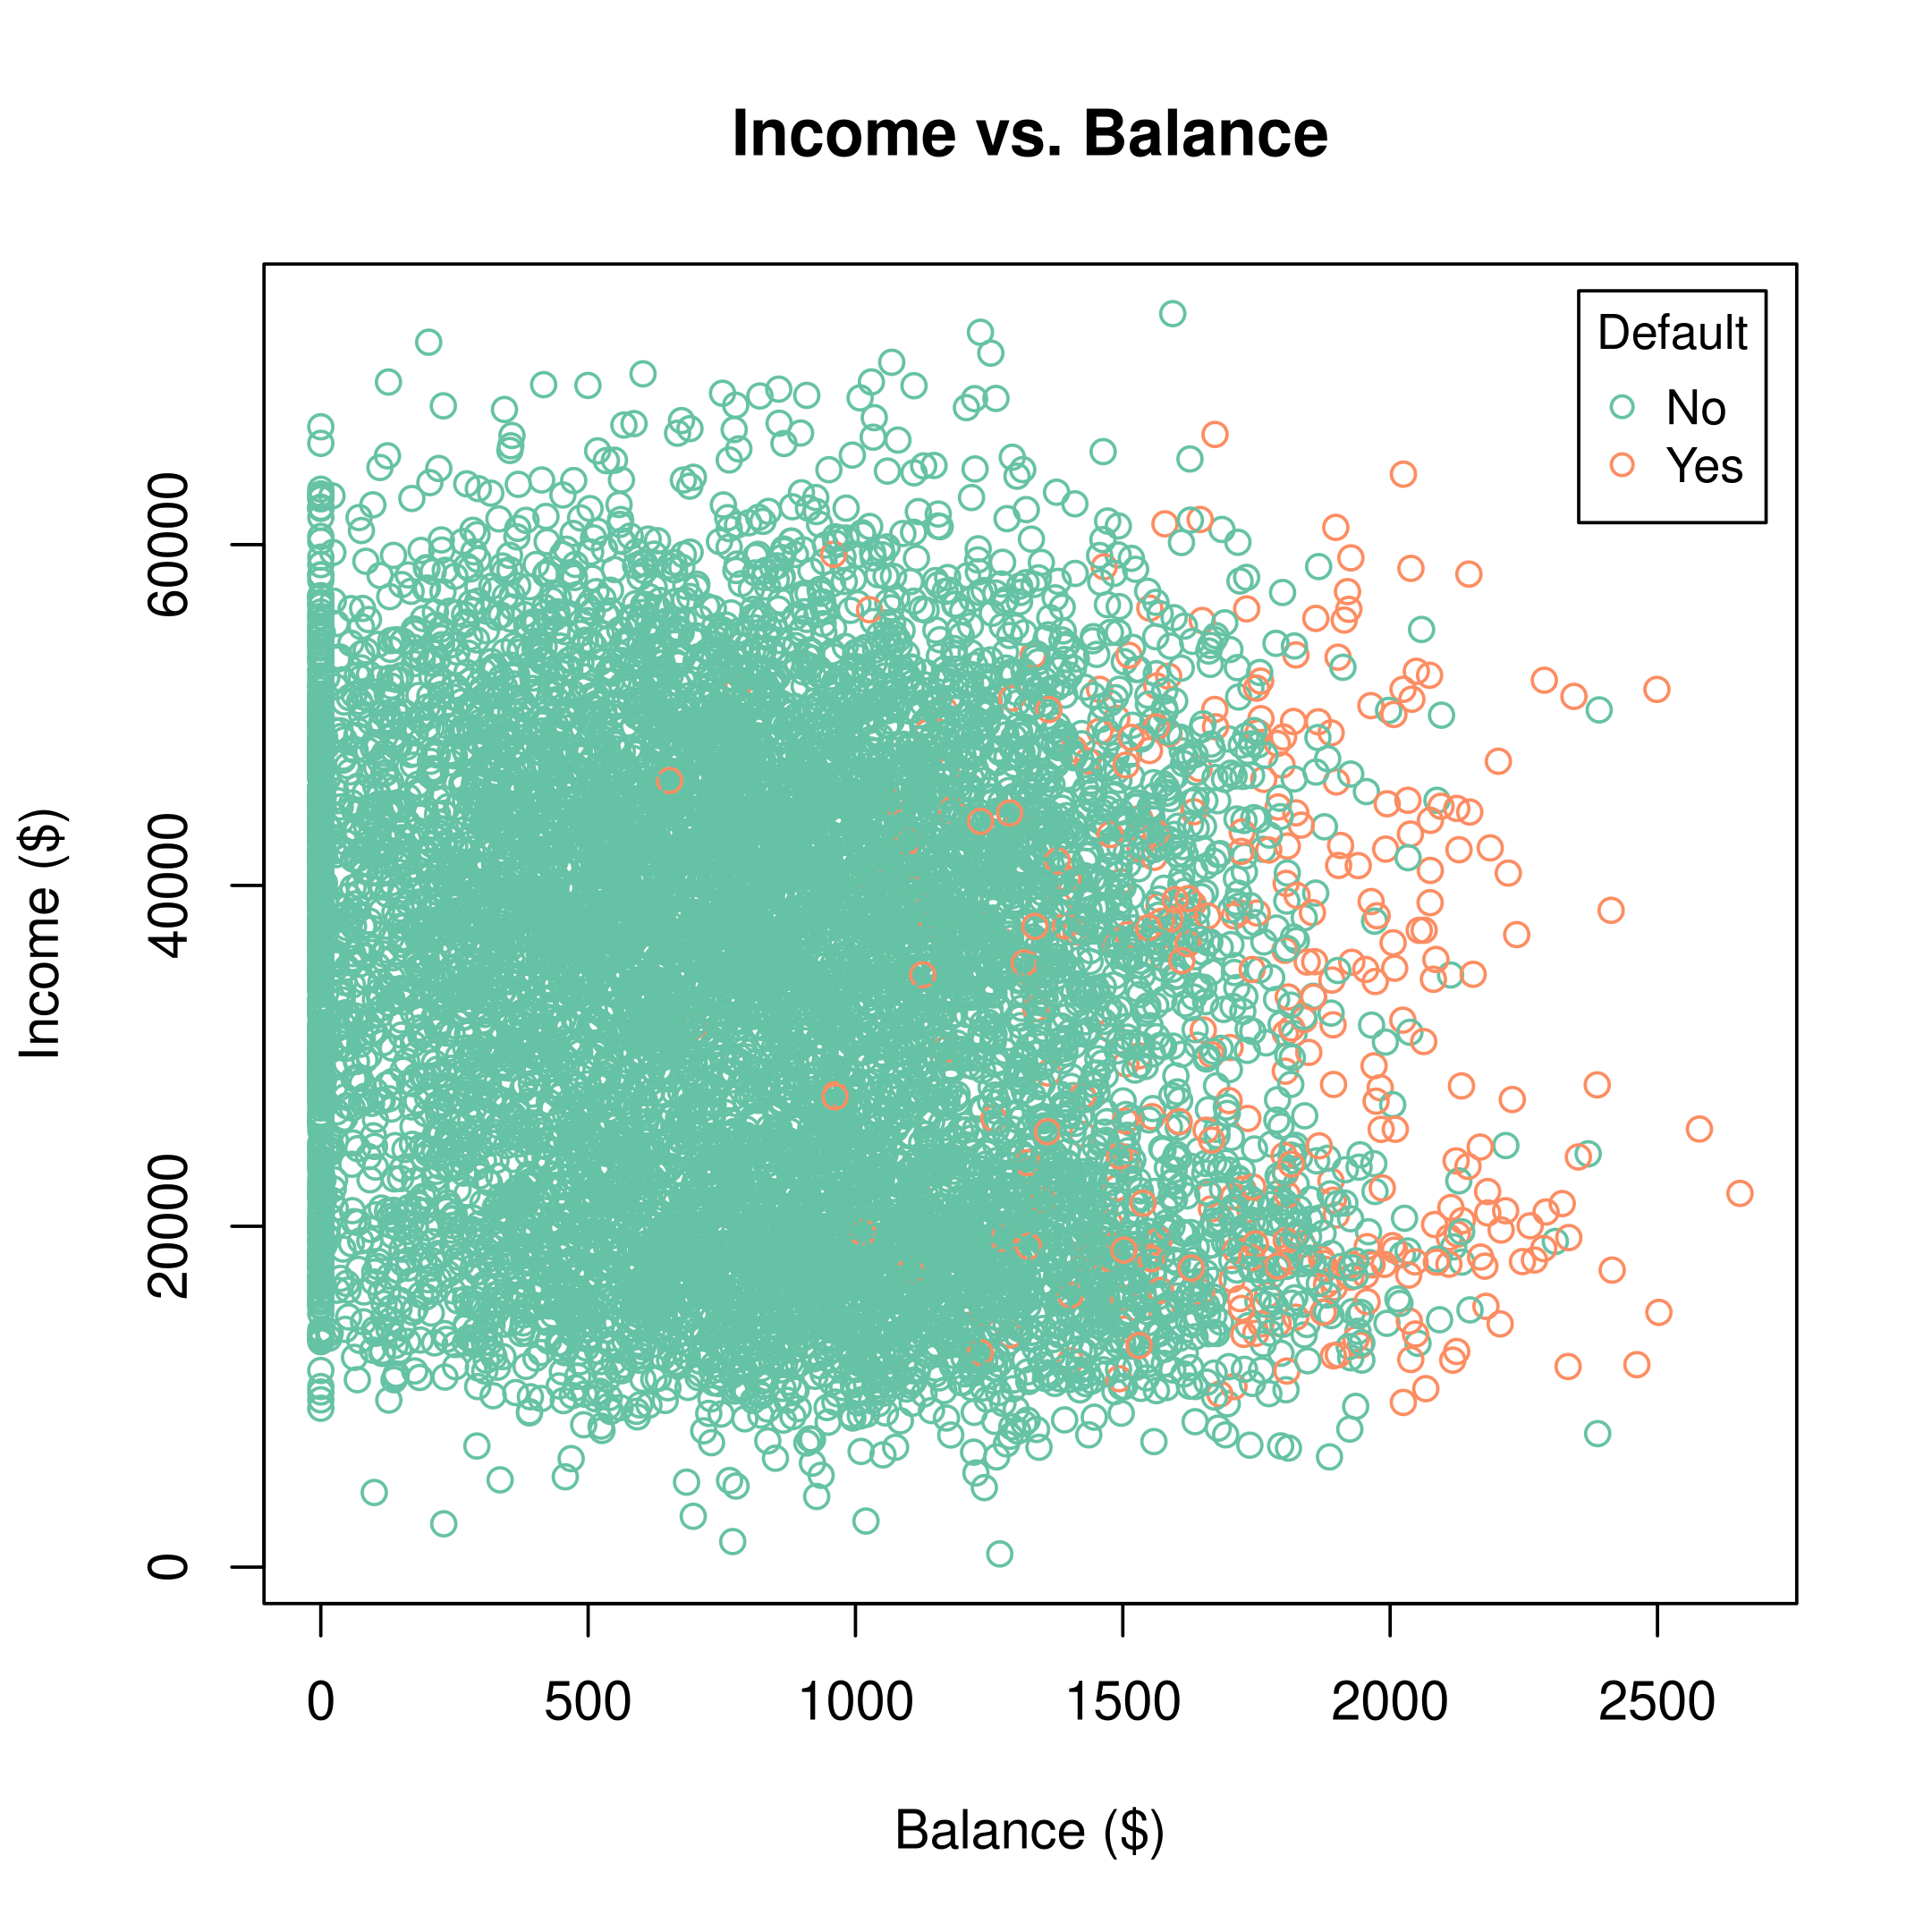
\includegraphics[width=.6\textwidth]{income-balance}
  \caption{Balance vs.\ income (Default dataset)}
  \label{fig:1}
\end{figure}
\begin{enumerate}[\bf (a)]
\item Estimate a logistic regression model to predict the probability of defaulting on credit card payments (assume \texttt{Default} = ``Yes'' is the positive class). \pts{3}
  Write down the estimated logistic function and comment on the significance of the parameter estimates.
\item Assuming a 50\% threshold,  use the logistic regression model to assign the default  status of the \pts{1} observations, i.e.:
  \begin{equation}
    \label{eq:3}
    \Pr(\mathtt{default = Yes}|\bm x) > 0.5
  \end{equation}
\item Generate a plot similar to that in \autoref{fig:1} \pts{3} and show the decision boundary at the 50\% threshold.
\item What are the overall error rate, sensitivity (recall) and precision of the classifier? \pts{3}
\item Tabulate or plot the confusion matrix. \pts{2}
\item How would you increase the sensitivity of your classifier? \pts{2}
  Indicate the action you would take and show the new decision boundary in the same plot generated in part (c).
\item Plot the receiver operating characteristics (ROC) curve based on the model \pts{2}
  estimated in \textbf{(a)} and state the area under the curve (AUC).
\item {\bf [Extra Credit]} What would be the shape of the ROC curve if the \texttt{default} response \pts{2}
  did not depend in any way on \texttt{balance} and \texttt{income}? Why?
\end{enumerate}  


\bigskip

% \section*{Problem 6 \quad {\it Cross-validation  (10 pts)}}
% Use $k$-fold ($k=5$ or $k=10$) cross-validation to compare the performance of the following models estimated to predict \texttt{Default} based on \texttt{income} and \texttt{balance}: KNN, logistic regression, LDA and QDA.
% Summarize your results (cross-validation scores/accuracy) using a table and a plot.


%\section*{Problem 6 \quad {\it Regression  and smoothing splines (20 pts; 5 pts EC)}}
% The objective of this problem is to apply a variety of modeling approaches to predict the \textbf{average} number of hourly
% bicycle pickups (\texttt{num\_pickups}) from bikeshare stations in Boston in 2017.  You will cope with overfitting and use
% regularization to counteract it.  You will also experiment with splines and smoothing splines.

% We will use the file \texttt{data/dataset-hubway.csv}.
% The data have been extracted from the opendata portal of the bikeshare service, Hubway
% \footnote{Note that Hubway is now called Blue Bikes. This dataset was extracted in 2018.} (\url{https://www.thehubway.com/system-data}).
% Each row contains information about the utilization of a single Hubway station in a 1-hour time window.\footnote{Note that you will have to aggregate the dataset to obtain the average hourly observations.} The variables are:

% \begin{enumerate}
% \item \textbf{Attributes related to the station and time}
%   \begin{compactitem}
%   \item \texttt{station\_id, year, month, day, hour} (hour of day)
%   \item \texttt{day\_of\_week}: from 1 (Monday) to 7 (Sunday)
%   \item \texttt{weekend}: 1 if Saturday or Sunday, 0 otherwise 
%   \end{compactitem}

% \item  \textbf{Supply and utilization information}
% \begin{compactitem}
%   \item \texttt{num\_pickups, num\_dropoffs}
%   \item \texttt{num\_bikes\_available, num\_bikes\_disabled, num\_docks\_available, num\_docks\_disabled} (on average during that hour)
%   \item \texttt{num\_bikes}: number of bikes, either available or disabled
% \end{compactitem}

% \item \textbf{Demographic information}
% \begin{compactitem}
% \item \texttt{TOWN} (Boston, Cambridge, Brookline or Somerville)
% \item \texttt{TAZ\_id}: TAZ stands for Traffic Analysis Zone. Each town is divided into serveral TAZes.
%   In this dataset, this variable refers to the TAZ in which the corresponding station is located.
%   \textit{All the subsequent attributes listed below are the TAZ-level characteristics.}
% \item \texttt{Tot\_Pop}: total population
% \item \texttt{HH\_Pop}: household population
% \item \texttt{HH}: number of households
% \item \texttt{Income\_low, Income\_mid\_low, Income\_mid\_high, Income\_high}:
%   number of households with a low, mid-low, mid-high or high income level
% \item \texttt{Worker0, Worker1, Worker2, Worker3p}: number of households with 0, 1, 2, 3 or more workers
% \item \texttt{HHSize1, HHSize2, HHSize3, HHSize4, HHSize5p}: number of households with size 1, 2, 3, 4, 5 or more 
% \item \texttt{Veh0, Veh1, Veh2, Veh3p}: number of households with 0,1,2,3 or more vehicles
% \item \texttt{Tot\_Vehs}: total number of vehicles
% \item \texttt{Age0to4\_enrollment, Age5to14\_enrollment, Age15to18\_enrollment}: Number of students, divided in age intervals
% \item \texttt{Age19plus\_commuters}: number of students 19 years old or older and commuters
% \item \texttt{Age19plus\_dorms}: number of students 19 years old or older in college dormitories
% \end{compactitem}

% \end{enumerate}

% In each exercise and sub-exercise, you can re-use models you already proposed (in other exercises in this present problem set or in the previous) or propose every time a new one, if you think it makes it easier to show what the exercise or sub-exercise is asking.

%Please note that you are free to perform the analysis for on a subset of the dataset. In this case, you should motivate your choice.

%\begin{exercise}{\it Validation and regularization in linear regression}



%\subsection*{Part 5.1 {\it Validation and regularization in polynomial regression and splines}}
 %  \begin{enumerate}[\bf (a)]
%   \item Choose \textit{one independent variable} to \pts{5} predict the average number of pickups per hour at a station.
%     Justify your selection.
%     Show the relationship of the independent variable to the dependent variable using a scatterplot.
%     Fit 3 regression splines on the training set with different degrees and knots.
%     %One of the splines you consider must have knots at all unique  points in the training set.\\
%     % NOTE: R may issue a warning at this point, saying that ``prediction from a rank-deficient fit may be misleading.''
%     % It means that there is multicollinearity in the model, and thus there are multiple solution of the regression problem
%     % (i.e., the minimization of the sum of the residuals squared).
%     % R is just choosing arbitrarily one of these solutions and using that for the prediction.
%     % You do not need to avoid this warning.
%     % If you get the warning, comment on it briefly and observe if the problems goes away with the regularization you will
%     % perform in the following sub-exercises.
 
% \item Plot the curves  \pts{3} that represent the 3 spline fits and comment on a visual comparison. Support your comments comparing the adjusted $R^2$ and some characterization of the coefficients, e.g., max and min.
  
% \item  Compare how well they predict the test set using a plot, table or both. \pts{2}

% \item Now, fit a \textbf{smoothing spline}  to the data. \pts{6}
%   Use cross-validation to select the ``best'' model (e.g.\ degree, etc) from a selection of possibilities.
%  % You have the liberty here to do an exhaustive search or choose a selection of possibilities to test.
%   Comment on the performance of your model.

% % \item Finally, fit a \textbf{smoothing spline} to the data. \pts{4pts} Use cross-validation to select the \textit{smoothness level} $\la$.
% %   The \texttt{smooth.spline()} function in the  \texttt{splines} (R package) has a built in \texttt{cv} option to implement this.
% %   Comment on the performance of your model.

% \item Plot the curves related to \textit{all} the models \pts{4}
%   you have estimated (along with \textit{all} the datapoints). Compare and contrast their test performance.
%   Summarize your overall findings.

% \item[\bf EC] Select other potentially relevant predictors and fit a multivariate smoothing spline or GAM to estimate the average number of hourly pickups. Compare the results of this new model to the best obtained in the univariate case. \pts{5}

% \end{enumerate}

% \section*{Problem 6 \quad {\it Generalized additive modeling (12 pts; 4 pts EC)}}
% Read the paper ``Estimating PM\textsubscript{2.5} Concentrations in Xi'an CityUsing a Generalized Additive Model with Multi-Source
% Monitoring Data'' (Song et al., 2015).

% The goal of this problem is to estimate a GAM model to explain the 2013 concentration of particulate matter
% (PM\textsubscript{2.5}) in Xi'an City, China, based on the presence of other atmospheric pollutants and the weather.
% The form of the model you are to estimate is given in by equation 2 of the paper (page 14). 

%    \begin{enumerate}[\bf (a)]
%    \item Estimate the GAM model described in the paper \pts{12} (reserving a portion of the dataset for performance
%      assessment purposes).  The authors state that the ``model explains 69.50\% of the total deviance in the
%      PM\textsubscript{2.5}'' data. Do your results match this performance? Explain why, if not.  Plot the performance of
%      your model on the test set (e.g.\ similar to Fig.\ 11b in the paper). Report key statistics from your model (e.g.\
%      MSE).

%    \item[\bf EC] See if you can improve the results reported in the paper by enhancing the model. \pts{4}
% \end{enumerate}
 
\end{document}

%%% Local Variables:
%%% mode: latex
%%% TeX-master: t
%%% End:
